\chapter{Dynkin Diagrams}
\label{ch-dynkin}

\newcommand{\valp}[0]{{\vec{\alp}}}
\newcommand{\vbeta}[0]{{\vec{\beta}}}
\newcommand{\vgamma}[0]{{\vec{\gamma}}}

This chapter is based on Ref.\cite{eli-daw-book}, section 20.4.

Lie algebra over reals (real vector space over generators $X_r$ for
$r=1,2, \ldots \cald$) $\cald=$  number  of real degrees of freedom, real dimension $\dim_\RR$
of Lie Algebra
\beq
[X_q, X_p] = \sum_t f\indices{_q_p^t}X_t
\eeq



\beq
g_{qs}= \sum_{p,t}f\indices{_q_p^t}
f\indices{_s_t^p}
=
\bcen
\xymatrix{
q\ar@{~}[r]
&f\ar@/_1pc/@{~}[r]
\ar@/^1pc/@{~}[r]
&f\ar@{~}[r]
&s
}
\ecen
\eeq

If $\det g =0$,

\beq
[X_a, X_b] = 0,
\quad
[X_q, X_p] =\sum_t f\indices{_q_p^t}X_t
\eeq

Can assume $\det g \neq 0$,
Cartan criterion (CC) for
group to be semi-simple.
If the CC is satisfied, can assume
$g_{st}$ is diagonal

\beq g_{s t}=\delta(s,t)=
\xymatrix{
\ar@{~}[r]&
}
\eeq

\beq
f\indices{_q_p^t}=f_{qpt}
\eeq
Will not choose $f_{qpt}$
to be totally antisymmetric


$q_- = 1, 2, \ldots,\calr$

$\valp = 1,2, \ldots, 
\cald-\calr$ 

$q=$ either $q_-$ or $\valp$ but not both.



Let $\{H_{i_-}\}_{i_-=1}^\calr$
be the largest possible set
of mutually commuting $X_p$.
$\calr$ is called the {\bf rank} of the group.

\beq
\boxed{[H_{i_-}, H_{j_-}]=0}
\eeq

Choose $E_{\vec{\alp}}$
to be eigenvectors of $H_{i_-}$ in the commutator \qt{product}
\beq
\boxed{[H_{i_-}, E_{\vec{\alp}}]= \underbrace{\alp_{i_-}}_{f_{i_-,\valp,\valp}} E_{\valp}}
\eeq


Then\footnote{The commutator $[x,y]=xy-yx$ acts like a derivative operator: 
$ [x[a,b]]= [[x,a],b] + 
[a,[x,b]]$}

\beqa
[H_i, [E_\valp,
E_\vbeta]]
&=&
[[H_i, E_\valp], E_\vbeta]
+
[E_\valp, [H_i, E_\vbeta]]
\\
&=&
(\alp_i + \beta_i)[E_\valp, E_\vbeta]
\eeqa

If $\valp + \vbeta=0$,
$[H_i, [E_\valp,
E_\vbeta]]=0$ so

\beq
\boxed{[E_\valp,
E_{-\valp}] = \sum_{i_-} \underbrace{\alp^{i_-}}_{f_{\valp,-\valp,i_-}} H_{i_-}}
\eeq

If $\valp + \vbeta\neq 0$,

\beq
\boxed{[E_\valp, E_\vbeta]=
 N_{\valp,\vbeta}
E_{\valp + \vbeta}
\quad \text{ if } \valp+\vbeta \neq 0}
\eeq


\beq
\alp^{i_-}=f_{\valp,-\valp,i_-} 
\eeq

Dynking Diagram (DD)

\beq 
n= \frac{-2 \valp\cdot \vbeta}{\valp\cdot\valp}
\label{eq-dynkin-n-pic}
\eeq

\beq 
p= \frac{-2 \valp\cdot \vbeta}{\vbeta\cdot\vbeta}
\label{eq-dynkin-p-pic}
\eeq

\beq
-\sqrt{
\frac{np}{4}}
=
\hat{\alp}\cdot\hat{\beta}\in [-1, 0]
\label{eq-dynkin-angles}
\eeq

\begin{figure}[h!]
\centering
\includegraphics[width=5in]
{dynkin/dynkin-constraint.png}
\caption{Pictorial representation of 
Eqs.(\ref{eq-dynkin-n-pic})
and (\ref{eq-dynkin-p-pic}).
}
\label{fig-dynkin-constraint}
\end{figure}

\begin{table}[h!]
\begin{tabular}{|l|l|l|}
\hline
\rowcolor[HTML]{FFFFC7} 
$np$ & $\sqrt{np/4}$ & $\arccos\left(-\sqrt{np/4}\right)$ \\ \hline
0 & 0 & $\frac{\pi}{2}=90^o$ \\ \hline
1 & $\frac{1}{2}$ & $\frac{2\pi}{3}=120^o$ \\ \hline
2 & $\frac{1}{\sqrt{2}}$ & $\frac{3\pi}{4}=135^o$ \\ \hline
3 & $\frac{\sqrt{3}}{2}$ & $\frac{5\pi}{6}=150^o$ \\ \hline
\end{tabular}
\caption{Possible root vector angles from Eq.(\ref{eq-dynkin-angles}).}
\label{tab-dynkin-angles}
\end{table}






\begin{figure}
\renewcommand{\arraystretch}{2}
$$
\begin{array}{ll}
 A_n=\ger{su
}(n+1)
& \dynkin[scale=3]A{}
\\
B_n=\ger{so}(2n+1)
& \dynkin[scale=3]B{}
\\
C_n=\ger{sp}(2n) 
&\dynkin[scale=3] C{}
\\
D_n=\ger{so}(2n) 
& \dynkin[scale=3] D{}

\\ E_6& \dynkin[scale=3] E6{}

\\ E_7& \dynkin[scale=3] E7{}

\\ E_8 &\dynkin[scale=3] E8{}

\\ F_4 & \dynkin[scale=3] F4{}

\\ G_2 & \dynkin[scale=3] G2{}

\end{array}
$$
\renewcommand{\arraystretch}{1}
\caption{Dynkin diagrams for the simple Lie groups}
\label{fig-dynkin-simple}
\end{figure}

\section{Examples}


\begin{itemize}
\item $SO(3)$ and $SU(2)$ have a single dot DD

\item $SO(4)\cong SO(3)\times SO(3)$ not a simple Lie algebra, its DD is two disconnected dots

\item For $SU(3)$

\beq
H_1=T_z,\quad H_2=\frac{\sqrt{3}}{2} Y
\eeq

\beq
E_\valp= \frac{1}{\sqrt{2}} T_+,
\quad
E_\vbeta = \frac{1}{\sqrt{2}} U_+,
\quad
E_{\vec{\alp}+\vec{\beta}}=\frac{1}{\sqrt{2}} V_-
\eeq


\begin{figure}[h!]
\centering
\includegraphics[width=2in]
{dynkin/dynkin-su3-roots.png}
\caption{Root system for $SU(3)$}
\label{fig-su3-roots}
\end{figure}


\end{itemize}



